% Options for packages loaded elsewhere
\PassOptionsToPackage{unicode}{hyperref}
\PassOptionsToPackage{hyphens}{url}
\documentclass[
]{article}
\usepackage{xcolor}
\usepackage{amsmath,amssymb}
\setcounter{secnumdepth}{-\maxdimen} % remove section numbering
\usepackage{iftex}
\ifPDFTeX
  \usepackage[T1]{fontenc}
  \usepackage[utf8]{inputenc}
  \usepackage{textcomp} % provide euro and other symbols
\else % if luatex or xetex
  \usepackage{unicode-math} % this also loads fontspec
  \defaultfontfeatures{Scale=MatchLowercase}
  \defaultfontfeatures[\rmfamily]{Ligatures=TeX,Scale=1}
\fi
\usepackage{lmodern}
\ifPDFTeX\else
  % xetex/luatex font selection
\fi
% Use upquote if available, for straight quotes in verbatim environments
\IfFileExists{upquote.sty}{\usepackage{upquote}}{}
\IfFileExists{microtype.sty}{% use microtype if available
  \usepackage[]{microtype}
  \UseMicrotypeSet[protrusion]{basicmath} % disable protrusion for tt fonts
}{}
\makeatletter
\@ifundefined{KOMAClassName}{% if non-KOMA class
  \IfFileExists{parskip.sty}{%
    \usepackage{parskip}
  }{% else
    \setlength{\parindent}{0pt}
    \setlength{\parskip}{6pt plus 2pt minus 1pt}}
}{% if KOMA class
  \KOMAoptions{parskip=half}}
\makeatother
\usepackage{graphicx}
\makeatletter
\newsavebox\pandoc@box
\newcommand*\pandocbounded[1]{% scales image to fit in text height/width
  \sbox\pandoc@box{#1}%
  \Gscale@div\@tempa{\textheight}{\dimexpr\ht\pandoc@box+\dp\pandoc@box\relax}%
  \Gscale@div\@tempb{\linewidth}{\wd\pandoc@box}%
  \ifdim\@tempb\p@<\@tempa\p@\let\@tempa\@tempb\fi% select the smaller of both
  \ifdim\@tempa\p@<\p@\scalebox{\@tempa}{\usebox\pandoc@box}%
  \else\usebox{\pandoc@box}%
  \fi%
}
% Set default figure placement to htbp
\def\fps@figure{htbp}
\makeatother
\setlength{\emergencystretch}{3em} % prevent overfull lines
\providecommand{\tightlist}{%
  \setlength{\itemsep}{0pt}\setlength{\parskip}{0pt}}
\usepackage{bookmark}
\IfFileExists{xurl.sty}{\usepackage{xurl}}{} % add URL line breaks if available
\urlstyle{same}
\hypersetup{
  hidelinks,
  pdfcreator={LaTeX via pandoc}}

\author{}
\date{}

\begin{document}

Paul Koop

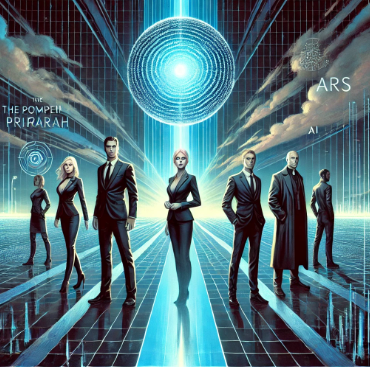
\includegraphics[width=4.92849in,height=4.92031in]{media/image001.png}

I.R.A.R.A.H. answers

The sequel to The Pompeii Project IRAHRA

Another short story about posthumanism

The team around Martina, Michael, Julia and Michael\textquotesingle s
doppelganger is led by I.R.A.R.A.H. rescued and has to survive a few
adventures in Germany, the USA and on the Ukrainian-Romanian border
before starting a new life in Budapest. Michael and his doppelganger
meet in Budapest.

Table of contents

\hyperref[disappeared-without-a-trace]{\textbf{Disappeared without a
trace 2}}

\hyperref[clothed-in-truth]{\textbf{Clothed in truth 18}}

\hyperref[escape-across-the-tisza]{\textbf{Escape across the Tisza 23}}

\hyperref[see-you-again-in-budapest]{\textbf{See you again in Budapest
29}}

\section{Disappeared without a trace}\label{disappeared-without-a-trace}

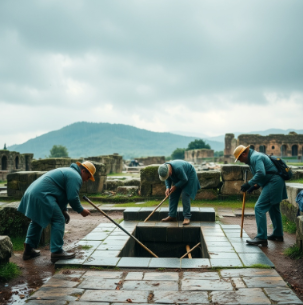
\includegraphics[width=4.11458in,height=4.09375in]{media/image002.png}

The rain fell in gentle, even drops on the excavation site in the
Archaeological Park of Pompeii. The earth beneath the
archaeologists\textquotesingle{} feet gradually turned into a viscous,
muddy mass, while the rhythmic ripples of water were the only sounds to
break the silence. Thick, gray clouds hung over the ruins, so deep that
they seemed to swallow the surrounding hills. The world seemed shrouded
in a damp veil, and the ancient walls and unearthed relics seemed even
more ephemeral, as if they could disappear back into the ground at any
moment.

Dr. Leonardo Moretti, the head of the excavations, stood leaning over a
crumbling stone wall, his gray eyes fixated on the progress of the work.
His weathered face was serious, and his thoughts wandered back to the
centuries when these streets and buildings had still been alive with the
people of Pompeii. The past few days had brought to light promising
finds - fragments of inscriptions and well-preserved household items
that revealed the everyday life of the ancient Romans. But today there
was a strange unrest in the air that couldn\textquotesingle t be
explained by the weather alone.

Suddenly an assistant hurriedly came towards him, his soaked clothes
clinging to his slim body and mud splashing with every step. ``Dr.
Moretti, the inscription is almost exposed. We need Martina Rossi for
the assessment,'' said the young man, his voice sounding quiet but
concerned.

Moretti looked up from the wall and frowned. Martina was the expert on
ancient writings; she was always called in as soon as a new inscription
became visible. "Where is she? ``She should be here by now,'' he
replied, his voice sharper than he intended.

The assistant shrugged, a nervous twitch crossing his face. ``Nobody saw
her today. ``She wasn't at breakfast either,'' he replied, avoiding
Moretti's gaze.

A strange feeling crept up inside Moretti, as if an invisible hand was
wrapping around his stomach and slowly squeezing it. Martina was
reliable, a woman who took every appointment and every task seriously.
The fact that she simply didn\textquotesingle t show up without giving
notice was unusual - too unusual to ignore. He looked at his watch. It
was almost midday. The rain continued to patter in steady drops on the
stone floor, and there was something oppressive about the darkness of
the clouds.

``I\textquotesingle m going to check on her,'' Moretti said finally,
more to himself than to his assistant, and looked over the excavation
site. His mind was already racing as he left the work area. He could
barely hear the other archaeologists\textquotesingle{} footsteps on the
wet stone as he walked away from the noise of the work. The remains of
the wall and rubble seemed to tower over him like silent witnesses to
his growing unease.

Moretti rushed to his car, which was parked at the edge of the
excavation site. He turned around briefly and saw the workers carrying
on under the protective tarpaulins, unfazed by the rain, which now
seemed to be easing. A light wind lifted the heavy clouds a bit, so that
the sky opened up and let a little light through. In his haste, Moretti
forgot his umbrella at one of the tables on the premises - a stupid
mistake, he now realized. As he made the short walk to his car, he
noticed the droplets from the tree leaves splashing onto his collar and
dampening his clothes. The cold crept through the fabric and made him
shiver slightly.

Inside the car, he revved the engine and turned on the windshield
wipers. The faint scrape of the wiper across the windshield mingled with
the constant ticking of the clock on the dashboard, which seemed
inexplicably eerie to him. Moretti felt the tension settle in his
shoulders. He thought of Martina and also of Julia, her friend and
roommate. Both were like sisters who seemed inseparable, even outside of
work.

What had happened? His head was full of chaotic thoughts, and the more
he thought about them, the more restless he became. Had they been
injured? Was there an accident? He dismissed the idea. He would have
heard if something had happened.

He took one last look at the area before turning onto the narrow,
rain-soaked street that led to Martina and Julia\textquotesingle s
apartment. The windshield wipers glided tirelessly across the glass as
he pressed the accelerator.

Moretti stopped in front of the small Italian house, whose facade was a
warm ocher and crumbling plaster. It was a familiar sight - a
nondescript building on a quiet side street in Pompeii that he had
visited many times before. But on this rainy day it seemed different, as
if an invisible threat had settled over the place. The shutters rattled
softly in the wind and the rain dripped down the edges of the roof as he
got out of the car. An uneasy feeling grew in his chest as he approached
the entrance, his footsteps echoing dully on the wet pavement.

Moretti hesitated for a moment in front of the door of Martina and
Julia\textquotesingle s apartment before he knocked decisively. His hand
trembled slightly as he pressed his fist against the dark wood. He
listened to the silence, hoping that at any moment footsteps would be
heard, that one of the women would open the door and greet him with an
apologetic smile. But it remained quiet. He knocked again, a little
louder this time, the tension making his voice echo louder in his head
than the hits on the wood. But even now everything remained quiet - no
noise from inside the apartment, no answer.

A feeling of apprehension ran through him, like a cold gust of wind
blowing through the half-open shutters. That didn\textquotesingle t sit
well with Martina. She was always organized, reliable, the kind of
person who had a plan for every occasion. Moretti glanced sideways and
saw a window that was slightly open. He stepped closer, the gentle sound
of rain and the distant hum of the city behind him fading into the
background as his attention turned fully to the interior of the
apartment.

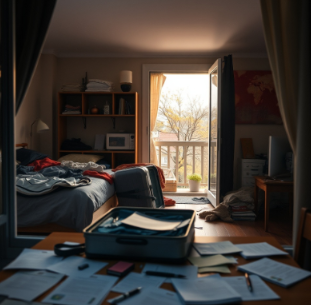
\includegraphics[width=4.14583in,height=4.11458in]{media/image003.png}

He peered through the crack in the window, and what he saw made his
heart beat faster. The interior of the apartment was a mess - clothes
were strewn across the beds as if they had been hastily rummaged
through. A half-packed suitcase stood in the hallway, crooked and open,
as if someone had left it in a hurry. Papers and notes were scattered
across the kitchen table, as if someone had been searching for something
important. There was something unreal about the scene, almost like a
staged picture, but the disarray spoke volumes of a sudden and
unprepared departure.

Moretti pulled away from the window, his heart pounding in his chest as
the reality of the situation hit him. ``That doesn't suit Martina.
She\textquotesingle s always so neat," he thought, worry building to a
pressure on his chest. A restlessness took hold of him that he could no
longer shake off. The scene inside the house sent shivers down his spine
as he wondered what could have happened.

His thoughts raced: Had they simply left everything there in a panic?
Was it an accident or something else, something darker, that had forced
her to disappear? He couldn\textquotesingle t make sense of it, but one
thing was clear: This was more than just a misunderstanding or an
oversight.

Impatience rose in him like the cold rainwater collecting on his shoes.
Moretti abruptly turned away from the door and ran quickly back to his
car. The sense of urgency was now gnawing at him relentlessly, like a
nagging pain that was becoming more and more intense. Without thinking
twice, he jumped into the car, revved the engine and drove off with the
tires spinning. The water splashed from the sides of the road as he
turned onto the wet, narrow street that led to the nearest police
station. His head was full of questions, but only one thing mattered
now: he had to get help, and as quickly as possible.

It was a gray, rainy morning when Dr. Leonardo Moretti stepped through
the heavy glass doors of the police station in Naples. The damp smell of
the city clung to his clothes, and his wet shoes squeaked softly on the
cool marble floor. The clouds hung low and gloomy over the city, as if
weighing down the life and hustle and bustle of Naples that could be
heard through the open windows - cars honking, street vendors shouting
and the quiet, steady sound of rain.

Moretti, his face tanned by the sun of past excavations and his hair
already graying at his temples, felt a lump in his throat. The unrest
that had accompanied him since morning had consolidated into a
frightening certainty. He walked quickly towards the reception desk,
where a young police officer was sitting behind a pile of files. The
archaeologist\textquotesingle s footsteps echoed through the room, each
step an echo of the pressing concern that had driven him here.

``I want to file a missing person report,'' Moretti said, his voice
urgent and sounding exhausted at the same time. He tried to remain calm,
but there was a hint of urgency in his words. ``Two of my colleagues --
historian Martina Rossi and her mother Julia Rossi -- have disappeared
since yesterday evening. You should be at the excavations this morning.
Your apartment...'' He paused for a moment, as if searching for the
right words. ``It's a mess, like they were in a rush.''

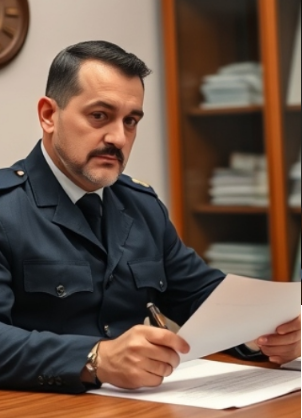
\includegraphics[width=4.0625in,height=5.61458in]{media/image004.png}

The policeman raised his eyes from the papers on his desk and gave
Moretti a searching look, then leisurely picked up a notepad and a pen.
``When did you last see them both?'' he asked matter-of-factly as he
slowly prepared himself for the protocol.

``Yesterday afternoon, at work,'' Moretti replied quickly. ``As always,
they were near the new excavation site. There was nothing unusual, no
signs that anything was wrong. But I didn\textquotesingle t hear from
them after that. They just... disappeared.'' Moretti\textquotesingle s
voice broke slightly, a rare tremble in his words that he
couldn\textquotesingle t suppress.

The police officer nodded and began to write down the information,
furrowing his eyebrows again as he wrote down the details. ``You say
your apartment was in disarray?'' he asked with a slight frown. ``Were
there any signs of violence or a struggle?''

Moretti shook his head. ``No, nothing like that. But it
wasn\textquotesingle t normal... the suitcases were half packed, clothes
were scattered everywhere, as if they were leaving in a hurry."

The policeman let the pen rest for a moment and looked at Moretti, as if
trying to fathom the meaning behind the archaeologist\textquotesingle s
words. ``We will file the complaint and begin the investigation
immediately,'' he said finally, in a tone that was probably intended to
be reassuring, but did little to change Moretti's nagging concern.

``Thank you,'' Moretti replied and nodded briefly, but his thoughts were
already on the next steps. What had happened to Martina and Julia? Every
second felt like it was filled with a thousand questions that he
didn\textquotesingle t have an answer to. As the policeman began to
delve into the depths of the bureaucracy to initiate the first measures,
Moretti felt the cold of the marble floor creep through his wet shoes,
as if the city itself was transmitting its gloomy mood into his heart.

He took a step back and looked around the station---officers hurrying
past him, telephones ringing, and the murmur of conversation mixing with
the sounds of the city streaming in through the windows. Moretti felt
strangely out of place at that moment. Here, in the world of order and
regulation, he could only hope that the restlessness in his chest would
soon give way to an answer. But when he wanted to leave the police
force, he knew deep down that this was just the beginning - the first
steps into a dark labyrinth where the disappearance of his colleagues
would potentially raise more questions than he could have ever imagined.

The police took the case seriously from the start. It was more than just
a routine procedure - it was the uneasy feeling that even the most
experienced officers couldn\textquotesingle t ignore when two people
suddenly disappeared without a trace. The police officer at reception
who had taken Moretti\textquotesingle s missing person report handed the
file with a curt nod to two investigators who specialized in such cases.
There was a sense of urgency in the air as the two officers, an older
man with salt-and-pepper hair and his younger colleague with a
determined expression, leafed through the file.

The office was hectic. The clatter of computer keys mingled with the
murmur of police officers and calls on phone lines as investigators
sorted through the details of the case. ``Two women, mother and
daughter, missing since last night,'' the older one read aloud.
``Apartment in chaos, no signs of a fight.'' He exchanged a meaningful
look with his colleague before resolutely swinging open the door of his
company car.

Just a few minutes later, the two investigators were already in the car
and driving through the rain-soaked streets of Naples towards Pompeii.
The sky was still covered in heavy clouds and the drizzle settled on the
windshield as the windshield wipers swung monotonously back and forth.
The journey was short, but in this short time a picture of the
possibilities was already formed in the minds of the two police
officers. It was her job to think through all the scenarios - and in
this area, where the shadows of the Camorra were omnipresent, there
could be many reasons why two women had disappeared without a trace.

When they reached the apartment building, the older investigator got out
and pulled his coat tighter around himself. The door to the apartment
was ajar, a detail that immediately caught his attention.
"That\textquotesingle s not good," he murmured, and his younger
colleague nodded as he pulled his gloves out of his pocket with a
practiced grip. They entered the apartment cautiously; the air was stale
and cold. The light was dim and the silence that hung in the room was
unnatural.

Clothes were strewn across the beds as if they had been hastily left
behind. A half-packed suitcase stood in the hallway, the lid open, and
one shoe lay lonely on the floor while its pair was nowhere to be seen.
There were open letters and notes on the kitchen table, some crumpled as
if someone had hastily thrown them away. The younger man bent down and
picked up one of the notes. ``It looks like you were in the middle of
preparing for a trip,'' he said quietly, dropping the note back onto the
table.

``That looks like a hasty departure,'' the older investigator murmured,
looking around the room. ``Clothes are lying around, the suitcases
aren't fully packed. But there are no signs of a struggle.'' He walked a
few steps further, opened a door that led to the bathroom, and found
nothing unusual there either. Everything seemed normal at first glance,
except for the disorder - an unexpected mess in an otherwise tidy
apartment.

The younger investigator went to one of the windows and pulled up the
blinds to get a better view. The daylight, albeit gray and dim, fell
into the room, illuminating the details of the disorder even more
clearly. ``Perhaps they fled or wanted to leave unnoticed,'' he said
thoughtfully. "There\textquotesingle s no indication that anyone took
her by force." He got down on his knees and examined the tracks on the
floor, but found nothing that suggested a fight or crime.

Back at the police station in Naples there was a tense atmosphere. The
two investigators gathered with other colleagues in a meeting room to
compile the findings so far. The possibility that this was an ordinary
missing person case was rapidly dwindling. There were too many
unanswered questions and the fact that the apartment was in such a state
gave them no peace.

``The whole thing is taking place in an area where the Camorra has a
hand in things,'' the older investigator remarked, casting a skeptical
look at the map hanging on the wall. ``It wouldn\textquotesingle t be
the first time that people disappear without a trace when they
unintentionally get involved in the machinations of local crime.'' His
colleague nodded in agreement. It was not an uncommon story of someone
being in the wrong place at the wrong time and then not being seen
again.

It was clear that this case went beyond the scope of normal
investigations. The decision to hand the case over to the public
prosecutor\textquotesingle s office was made quickly, and the Direzione
Distrettuale Antimafia, which was responsible for organized crime, was
also involved. Too many questions remained unanswered, and the idea that
there could be more to the women\textquotesingle s disappearances kept
investigators from thinking.

As officers at the police station worked frantically to secure initial
leads and interview witnesses, the uneasy feeling grew that they were
dealing with a case that was darker and more dangerous than it first
appeared .

There was a depressing silence in the DA\textquotesingle s office as the
prosecutor, a middle-aged man with deep lines around his eyes and a
frown borne of years of sleep deprivation, leafed through the initial
reports. The piles of files in front of him seemed to be pulsating, the
situation was so urgent. ``A case like this near Pompeii could well be
connected to the local Camorra,'' he murmured, his voice calm but firm.
He placed the report on the table with a thud and looked at the
assembled investigators one by one. ``We have to follow every lead --
bank details, phone activity, contacts. Check whether they have recently
withdrawn large amounts or made any unusual purchases. No detail is too
insignificant.''

The investigators stood tensely, the air in the room seemed to become
heavier. One of the younger officers stepped forward, his eyes
determined. ``Your workplace has officially confirmed the missing person
report. The colleagues at the excavations are extremely worried. I
suggest we investigate there thoroughly again. There could be clues we
missed.''

The prosecutor nodded in agreement. ``Good, do that. And I want the
Direzione Distrettuale Antimafia (DDA) to be involved. If the Camorra
has a hand in it, we need the best people on this case.'' He stroked his
unshaven chin and thought for a moment. ``And keep an eye out for
anything that might be related to historical artifacts. There are many
valuable excavations in the area that could attract the interest of
organized crime.''

While the investigators were receiving their instructions, they were
already reaching for their cell phones to organize initial interviews
and take the next steps. They knew they were under a lot of pressure -
not just because two people were missing, but also because there was
more at stake: power, history and perhaps even life and death.

Meanwhile, ARS, the artificial intelligence operating secretly for
I.R.A.R.A.H, was preparing its next digital deception. It was as if ARS
had already anticipated that the authorities would dig deeper. In the
police and airline networks, their algorithms worked quickly and
efficiently. Flight and travel records were manipulated or deleted,
bookings were canceled and passenger lists were falsified. It now looked
as if Martina and Julia had never left the city. Artificial intelligence
concealed the evidence so thoroughly that even experienced investigators
were caught in a thicket of false leads and misleading information.

But the authorities were not so easily discouraged. The suspicion that
the two historians might have discovered something that
shouldn\textquotesingle t come to light seemed too concrete to simply
dismiss. A few days later, after investigators reexamined the excavation
site and conducted further interviews, they uncovered a new clue. During
a thorough search of Martina and Julia\textquotesingle s apartment, they
found a business card - Michael Phillips, professor at the Gregoriana in
Rome.

The investigators looked at the map thoughtfully. ``Who is this man and
why did you have his business card?'' one of the officers asked loudly.
The fact that Michael Phillips worked near the Vatican made her sit up
and take notice. It was a connection that could have meaning in many
ways. The proximity to Rome\textquotesingle s religious and academic
elite, the connections to the intellectual world - everything suddenly
seemed important.

A call was made and shortly afterwards a team was assembled to be sent
to Rome to speak to Michael Phillips. The investigators carefully
prepared their questions, gathering information about the professor and
his work so as not to give him an opportunity to escape during
questioning.

Meanwhile, Michael Phillips sat in his office at the Gregoriana. It was
a warm, quiet room decorated with bookshelves that stretched from
ceiling to floor. The light from his desk lamp cast long shadows on the
wooden table. He felt as if these shadows were moving closer and closer
to him. For days he had felt the tension growing around him, like a web
that was slowly but inexorably tightening. The investigation in Naples
had gained momentum, and he knew that Martina and Julia were now the
center of the authorities\textquotesingle{} attention - and with it he
too.

An encrypted message from ARS had recently arrived on his laptop. ``The
air traffic control entries were successfully deleted. No more traces in
the databases,'' he read on the screen. There was a kind of relief that
coursed through his body, but it was fleeting. The pressure
didn\textquotesingle t decrease; On the contrary, he grew with every
passing minute, knowing that the slightest mistake could jeopardize
everything.

As dusk fell over Rome, Michael continued to sit at his desk. The sounds
of the city came through the open window: the hum of the streetlights,
the sound of engines in the distance. It seemed like an oppressive
crescendo that made his thoughts whirl faster and faster. He knew the
investigators would arrive soon. The game had started and he had to make
sure I.R.A.R.A.H wasn\textquotesingle t exposed. It was a risky game -
one with the safety of Martina and Julia at stake.

As he waited for the moment when there would be a knock on his office
door, Michael leaned back and let his gaze wander over the spines of
books on the shelves. There were works on philosophy, theology, and
history, but now they all seemed irrelevant given what was at stake in
the next few hours.

The knock on the door made him jump. The time had come. The
investigators were there, and Michael knew that every word he was about
to say would be watched and analyzed like a hawk.

A loud knock on the door broke the silence in the room, making Michael
Phillips jump. He had been expecting this moment, prepared to put on the
perfect mask. But he still felt the uneasy knot in his stomach that just
couldn\textquotesingle t be dispelled. Taking a deep breath, he stood up
slowly, forcing himself to remain calm as he walked to the door and
opened it.

Two men in dark suits stood before him, one with a stern, unmoving
expression on his face, while the other kept his expression more
relaxed, but in his eyes there was the cold, focused sharpness of a
hunter. ``Dr. ``Phillips?'' said the first with a hint of emphasis in
his voice. ``We are from the Polizia di Stato. It\textquotesingle s
about an interview about the disappearance of Martina Rossi and Julia
Rossi. Can we come in?''

Michael nodded silently and stepped aside to let her in. The men entered
his office and he could feel the cautious tension in their movements. It
was as if they were registering every wrinkle in his face, every
involuntary gesture. He led them to a small, round table in the middle
of the room and sat down while the investigators took their seats. The
serious policeman sat down directly in front of him and fixed him with a
penetrating gaze, while the other remained at the edge of the room,
attentive, scanning every corner of the office with his eyes.

``We have some questions for you,'' the police officer began, opening
his notebook. ``You know Martina Rossi and Julia Rossi very well,
don\textquotesingle t you?'' His voice was calm, but there was an
unspoken distrust behind it.

``Yes,'' Michael replied calmly, his hands resting on the table as he
returned her gaze. ``I worked with them on various projects, both
academic and within InSim.''

The policeman nodded curtly, as if he already knew. ``Martina's employer
filed a missing person report. She was last seen near you. Can you tell
us what happened the day she disappeared?''

Michael took a moment before answering, sorting his thoughts carefully
so as not to give any unwanted clues. ``I remember we met before she
left for Pompeii. They wanted to go back to Italy for a workshop.
Everything seemed completely normal.''

The two men exchanged a quick look, and the policeman leaned forward
slightly, as if to observe Michael\textquotesingle s expression more
closely. ``Normal?'' he asked with a hint of skepticism in his voice.
``There were no signs that anything was wrong?''

Michael shook his head calmly, careful not to seem too eager. ``Nothing
that I noticed,'' he replied evenly. But inside he fought to push away
the uneasy feeling. At this moment, ARS\textquotesingle s invisible
interface hummed softly in his ear. The AI's voice sounded like a
whisper from another world: ``They are checking aircraft records. We
deleted them. Stay calm."

The investigator continued to fix him with his penetrating gaze. ``And
what do you know about the InSim Mercedes accident that crashed near
Pompeii? Two witnesses claim the vehicle was followed by an unknown
group.''

Michael felt a light sheen of sweat appear on his forehead, but he
forced his expression to remain calm. ARS responded immediately and sent
a reassuring message: ``We have processed the surveillance data from the
accident. They will find no further evidence.''

``All I know is that they were on their way to a conference,'' Michael
said with as much composure as he could muster. ``The accident was
unexpected. I was in Rome at the time.'' He hoped his voice sounded calm
enough, even if he felt the pressure growing inside to weigh every
detail perfectly.

The policeman watched him for a few seconds longer, as if he wanted to
see something in his eyes that Michael wasn\textquotesingle t revealing.
Then he reached into his jacket pocket and pulled out a business card,
which he placed on the table in front of Michael. The card seemed small
and inconspicuous, but its significance was profound. It was
Michael\textquotesingle s own business card. ``This card was found among
the women's personal belongings,'' the investigator explained calmly.
``Can you explain that?''

``Yes, that's my card,'' Michael replied without hesitation. ``I gave
them to both of them in case they wanted to contact me for academic
questions. They've had a lot of technical questions lately that they
wanted to clarify.''

A deep silence spread across the room, as if the air itself had become
heavier. Michael felt the tension building, felt the investigators
waiting, as if they were waiting for him to make a mistake. He held his
nerve, forcing himself to hide any trace of nervousness. The gentle hum
of ARS\textquotesingle s voice remained constant in his ears, a
constant, soothing companion in this dangerous game.

After what seemed like an endless minute, the second investigator stood
up and walked to the window. He did it casually, but Michael noticed the
alertness in his movements, as if he was searching for something. ``You
don't know anything about your current whereabouts?'' he asked over his
shoulder. ``Any clues as to where they might be?''

``Unfortunately not,'' Michael replied calmly. ``I'm worried about her
too.''

The second investigator came back, leaned over the table and fixed
Michael with a piercing gaze that left no room for doubt. ``If you are
hiding something from us, Dr. Phillips, we\textquotesingle ll find out.
You know that.''

Michael smiled thinly, even as his stomach churned with tension. ``I
understand,'' he said calmly. ``You can contact me again at any time.''

The two men got up and left the office, but their suspicious looks
remained on Michael long after the door had closed behind them. He sank
heavily into his chair, his muscles relaxing slowly as the adrenaline
wore off. ``They left. The tracks are covered. Martina and Julia are
safe,'' ARS whispered in his ear, a gentle breath of relief.

Michael closed his eyes and took a deep breath. But the worry remained,
buried deep within him - a constant companion reminding him that they
were all just a small step away from being exposed.

The monastery of the Congregatio Jesu, located on the quiet
Maria-Ward-Strasse in Simbach am Inn, was once a lively place. The
voices of students and teachers used to echo in the corridors, full of
life and thirst for knowledge. But those days were long ago. Now the
monastery was almost deserted, the buildings stood silent and deserted,
as if in a deep slumber from which they would soon not awaken. The
impending closure seemed inevitable; the old walls no longer met modern
fire protection regulations. But it was this isolation and the
dilapidated tranquility of the forgotten place that made the monastery a
perfect hiding place for those who needed to escape the watchful eye of
the world.

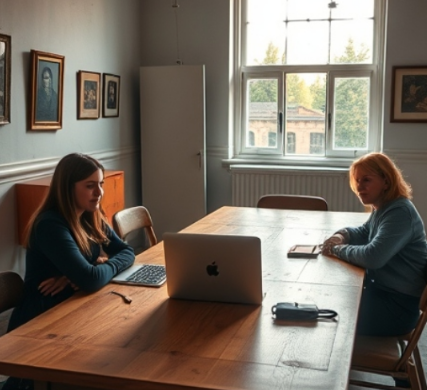
\includegraphics[width=5.65625in,height=5.25in]{media/image005.png}

In one of the former classrooms, which had been temporarily converted
into a meeting room, dust hung heavily in the air. Faded paintings and
photographs commemorated Maria Ward and the school\textquotesingle s
history lined the walls, while the long wooden table in the center of
the room towered over everything. A laptop sitting on the table was
already equipped with an encrypted connection, waiting to connect the
key participants in this secret meeting. Martina and Julia sat on one
side of the table, their faces serious and tense. The light of the late
afternoon sun shimmered through the half-open blinds, casting a
flickering play of shadow and light on their faces.

At the other end of the room, Michael\textquotesingle s doppelganger
leaned silently against the wall, his face half hidden in the dark. He
stood still, almost motionless, like a statue watching over the scene.
The only sounds were the gentle ticking of an old wall clock and the
occasional creaking of the floorboards, which only added to the eerie
silence.

Suddenly the laptop screen flickered and the faces of ARS and Michael
Phillips appeared, along with the serious face of the I.R.A.R.A.H
operator who would be leading this meeting. ARS\textquotesingle s
projection seemed almost alive as the AI \hspace{0pt}\hspace{0pt}spoke
in a voice that sounded soothing but cool at the same time. ``Welcome,''
ARS said, her tone seeming to pierce the silence of the room.
``It\textquotesingle s good that we can meet in such a secluded place.
The situation requires the utmost discretion.''

Michael Phillips\textquotesingle{} face, connected from Rome, appeared
tense, his eyes scanned the group and briefly rested on each individual.
``The situation is getting worse,'' he began in a serious voice that
brooked no contradiction. ``Professor Neumann in Kassel has already
received several threatening letters. His public lecture tomorrow could
lead to escalation. We must get him to safety before it is too late.''
His words hung heavily in the room, and for a moment it seemed as if
time itself was holding its breath.

Martina and Julia glanced at each other quickly, their gazes full of
unspoken questions, before returning their attention to the screen. ARS
took the floor and began a presentation that detailed the situation in
Kassel. The images flashed across the screen - security footage of
demonstrators waving protest signs and chanting angry slogans outside
the university entrance. Faces full of anger and determination that
posed a vague threat to the Professor and everything he represented.

``Professor Neumannt is a respected scientist,'' explained the
I.R.A.R.A.H operator, whose serious face remained almost motionless.
``He is known for his critical attitude towards postmodern trends and
transhumanism, which he sees as a threat to basic democratic values. Our
job is to get him out of the university and placed somewhere safe before
the situation gets out of control.''

Julia hesitantly raised her hand and asked with a hint of concern in her
voice, ``What if they spot us on the way?'' Do we have a backup plan?"

Michael responded from Rome, his voice firm and determined: ``Yes, ARS
has identified several alternative routes. In case we cannot get to the
chapel on the university campus as planned, there are underground
passages that date back to the Second World War. I.R.A.R.A.H has also
prepared a safe hiding place in a remote chapel on the outskirts of
Kassel.''

A map of the city of Kassel appeared on the screen, interspersed with
intricate lines indicating possible escape routes. ``Some local
supporters will organize diversionary tactics,'' ARS continued. "If
escaping the campus becomes difficult, we can trigger spontaneous
demonstrations elsewhere in the city to distract the authorities." The
artificial intelligence seemed to take every eventuality into account,
and the cold precision of its voice reinforced the impression that There
was no room for error here.

The I.R.A.R.A.H operator leaned closer to the screen, as if to emphasize
the seriousness of his words. ``During the mission, all communication
will be heavily encrypted and will pass through special devices that you
will carry with you. The risk remains high, but we are prepared.'' His
voice was calm but firm, like that of a commander sending his soldiers
into battle.

Michael\textquotesingle s doppelganger took a step closer to the table,
his figure standing out sharply against the shadows that filled the
room. ``After rescuing the professor, we should first bring him here to
the monastery,'' he suggested. ``The dissolution of the monastery is
delayed and the building is surrounded by a park. A safe place, at least
for a few days.''

ARS nodded slightly, the projection on the screen seemed to come alive
for a moment. ``The monastery offers a strategic position,'' the AI
\hspace{0pt}\hspace{0pt}said. ``I will increase surveillance and ensure
any movement around the site is captured.''

Finally, Michael Phillips raised his voice again, his words sounding
like an appeal to everyone present: ``Remember,'' he said urgently,
``this rescue is more than just an escape operation.
It\textquotesingle s about standing up for freedom of thought, for the
right to seek the truth. Every step can decide whether we win or lose.''
His words left a lasting impression, the silence afterwards was almost
noticeable.

After a moment that felt like an eternity, ARS concluded the briefing.
``The mission is risky, but our planning and flexible responses give us
the best chance of success. I will support the team around the clock.''
The AI's words continued to resonate as the screen faded.

The briefing was over and the team began final preparations. As they
left the meeting room, it seemed as if the weight of the task ahead was
weighing on their shoulders. The old corridors of the monastery, once
filled with youthful life, now seemed like silent sentinels, keeping the
secret of the planned rescue safe. But outside these walls there was a
dangerous world that had no regard for mistakes or insecurities.

\section{Clothed in truth}\label{clothed-in-truth}

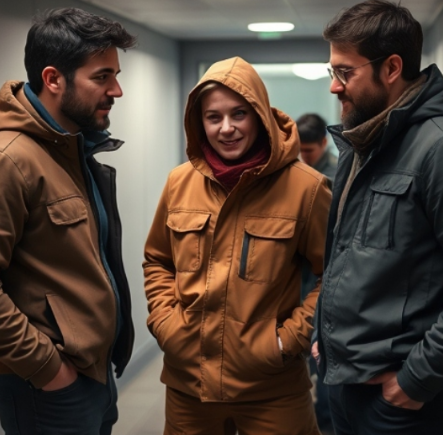
\includegraphics[width=5.88542in,height=5.79167in]{media/image006.png}

The morning was cool and foggy when Julia, Martina and
Michael\textquotesingle s doppelgänger arrived on the Kassel University
campus. A leaden haze hung over the buildings, and the tense atmosphere
was almost palpable. The day didn\textquotesingle t start like any
other, and they felt it in their bones. Already in the distance they saw
the first protest signs raised into the cloudy sky: ``Against fascism
and enemies of science!'' and ``Away with the reactionary!'' echoed from
a group of demonstrators who had gathered in front of the main building.

``It won't be easy,'' Julia whispered, looking around with a worried
expression. Her eyes scanned the crowd, packed into an angry mosaic of
faces and signs.

``We have to hurry,'' said Michael's doppelganger, straightening his
shoulders as they stood like a shield against the approaching cold.
``The professor is waiting for us. The quicker we get him out of here,
the less chance they have of recognizing us.''

Martina nodded and cast a searching glance at the gray clouds that
covered the sky as if they were summoning some unwritten omen.
``I.R.A.R.A.H has prepared everything. Let's not waste any time.''

They slipped discreetly into one of the outbuildings, their steps quick
but controlled. The sound of protests outside grew louder, but inside
the university building was quiet. The contrast felt surreal. In the
sparsely furnished office they found Dr. Tobias Neumann, who was
hurriedly packing his things into a worn leather bag.

He was a middle-aged man, with sharp features and a look of exhaustion
and determination in his eyes that lay deep in their sockets like two
shadows in a dark alley.

As the team entered, he looked up and breathed a sigh of relief. ``I've
been waiting for you,'' he said and put the bag down. ``The situation
outside is getting worse. The demonstrators are particularly aggressive
today.'' His voice was a rough thread that ran through the tense air.

``We have everything prepared,'' said Michael's doppelganger calmly,
taking a brown Franciscan habit out of his pocket. ``Here is your
religious habit. As soon as you put it on, you are officially Brother
Timothy -- a Franciscan on his way to the USA.''

Martina handed him a fake ID card. ``I.R.A.R.A.H made sure you had a new
identity. Your religious name and your new existence are secured.'' The
words weighed heavily on the professor's shoulders, who felt the weight
of his situation.

Dr. Neumann stared at the habit before standing up resolutely. ``This is
crazy,'' he muttered as he wrapped himself in the brown habit. ``But I
have no choice.''

As soon as he was finished, they led him outside through the empty
hallways of the university building. An inconspicuous van was parked in
front of the door, but getting there was not without risk. The protests
outside the university had become louder, and the crowd seemed heated
about the professor\textquotesingle s upcoming lecture.

``We have to get through this,'' Julia said, scanning the crowd. ``They
mustn't notice that it's you. We only have a short time.''

``I will go ahead with him,'' said Michael's doppelganger resolutely.
``You should believe we are a group of Franciscans on a pilgrimage.''

Dr. Neumann shook his head as they slowly moved toward the crowd. ``It's
crazy what these groups have become,'' he whispered. ``They used to be
intellectual. Today they are paid demonstrators from left-wing
communities who are here just to cause a ruckus.''

The protesters barely noticed them as they pushed their way through the
crowd. Some shouted insults, others raised their signs, but no one
seemed to recognize them. But then, just before they reached the van,
there was a shout from the crowd: ``That's him! The reactionary
professor!''

The protesters\textquotesingle{} eyes turned to her, and for a moment it
seemed as if the situation was escalating. The crowd\textquotesingle s
pulse quickened like the roar of an approaching storm. But
Michael\textquotesingle s doppelganger pushed Dr. Neumann quickly into
the van. The door closed with a thud and they drove off, angry shouts
ringing out behind them.

On the motorway to Frankfurt it was quiet in the car, but the tension
was still palpable, like a rope being overstretched. The professor
leaned back and sighed heavily, the pressure on his chest seemingly
easing momentarily. ``Discussions used to be possible,'' he said
thoughtfully. ``Today all I see is anger and ignorance. Antifa was once
an intellectual movement, but now it has become an instrument of hate.
They are paid to silence those who think differently.''

``You're no longer interested in arguments,'' Martina agreed. ``It's
just a matter of destroying the enemy.''

``It's a sad development,'' Michael's lookalike added. ``But in the USA
you will have a new chance. There you can speak freely without being
threatened by cancel culture.''

The professor nodded, but his thoughts still seemed to linger on the
events in Germany. ``It\textquotesingle s hard to believe how quickly
things have changed. We have surrendered our critical thinking to
technology. I hope to be able to save something in the USA.''

When they arrived at Frankfurt Airport, the team led the professor
through security checks. Every step had to be planned precisely because
a single mistake could jeopardize their entire operation. Julia glanced
over her shoulder as the professor handed his papers to the security
guards. It only took a moment, but what seemed like an eternity, for the
officer to wave him through.

``Once you're in the US, you're safe,'' Julia said, putting a hand on
the professor's shoulder. ``I.R.A.R.A.H will take care of everything
else.''

Dr. Neumann nodded, a hint of gratitude in his eyes. ``Without your help
I would have been lost,'' he said quietly. ``I owe you my life.''

They watched him go through the gate and the flight to Chicago was
called. They took one last look at the man they had saved before he
disappeared behind the glass doors.

Once in the United States, the professor was picked up by a member of
the Franciscan community and taken to the Franciscan University of
Steubenville. The team accompanied him on the long journey to the
university, whose calm and peaceful atmosphere contrasted with the
chaotic conditions in Germany. The trees that surrounded the campus
acted like silent sentinels, protecting the new arrivals.

``Welcome, Brother Timothy,'' one of the brothers greeted him with a
warm smile. ``Your reputation precedes you. We look forward to welcoming
you to our community.''

"It will be an honor," the professor replied, nodding slightly, the
weight of his new identity feeling both liberating and oppressive.

The day after his arrival, the professor gave his inaugural lecture to
an assembled group of Franciscans and students. The team sat at the back
of the room and listened intently as the professor chose his words
carefully. The auditorium was filled with a quiet anticipation, the air
seemed to vibrate as he spoke.

``At a time when people are handing over their responsibility to
technology,'' he began, ``we must return to the values
\hspace{0pt}\hspace{0pt}of enlightenment and rationality. It is not
technology that will save us, but critical thinking. We must defend
humanism against postmodern trends.''

The words echoed in the room, and for a moment it seemed as if the sharp
edges of the world outside no longer had any power over her. A
collective nod went through the ranks, the students seemed to sense the
spark of hope that lay within the professors. But the reality
couldn\textquotesingle t be ignored for long.

After the lecture, Martina, Julia and Michael\textquotesingle s
doppelganger met with an I.R.A.R.A.H agent in one of the back rooms of
the university. The agent was a slim man with a serious expression,

who sat across from them as they shared their impressions of what had
happened.

``It was risky,'' the agent said, his voice calm and controlled. ``But
we have information that some of the demonstrators in Germany have the
goal of also infiltrating the Franciscan community. It could be that she
is referring to Dr. Neumann are out.''

``What can we do?'' Julia asked worriedly.

``We must ensure the safety of the professor and strengthen the
connection with the community. He has become a target. The question is
not if they will try to find him, but when.''

``That means we have to strengthen the defense,'' Martina added. ``He's
not just a professor. He is a symbol.''

The agent nodded. ``Over the next few weeks, it will be crucial to
secure our communications and keep an eye on movements in the community.
It will take time to smooth out the waves that the events in Germany are
bringing here.''

The next few days were characterized by intensive discussions about
strategies to maintain the professor\textquotesingle s safety.
Meanwhile, Dr. Neumann, how he gradually grew into his new identity. He
found that he had a voice that wanted to be heard in the new world - and
he was encouraged by the opportunities he had here.

He gave lectures once a week and the auditorium filled with students who
listened eagerly to his ideas. He remembered again and again the
coldness of the demonstrations in Germany, the threats that had
imprisoned his mind, and the heated debates that never led to anything.
Here discussion was possible again and people\textquotesingle s hearts
were ready to open themselves to the ideas of humanism.

One evening, after a particularly encouraging talk, he sat at the table
with his new brothers. ``I never thought I would be so alive,'' he said,
raising his glass. ``To freedom of spirit!''

``To freedom of spirit!'' the others shouted in unison, and a feeling of
community filled the room.

Dr. Neumann felt free for the first time in a long time, and when he
looked at his brothers\textquotesingle{} faces, he knew he was safe. The
shadows of the past seemed to fade as he walked the new path that lay
before him.

In this new world he could share his knowledge and passion for the truth
without fear of persecution. People no longer needed censorship, but
rather the courage to stand up for the truth. And while darkness still
raged in Germany, hope bloomed in the halls of Franciscan University.

\section{Escape across the Tisza}\label{escape-across-the-tisza}

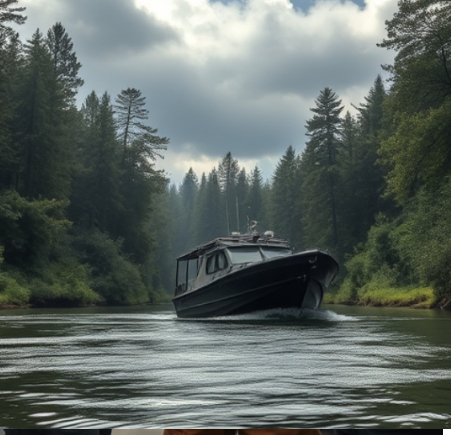
\includegraphics[width=6in,height=5.78125in]{media/image007.png}

It was still early in the morning when the team gathered in the briefing
room at Franciscan College in Steubenville. The first rays of sunlight
broke through the morning light and bathed the room in a soft gold, but
the atmosphere was anything but relaxed. A bright neon light flickered
above the table, which was littered with documents and notes. The air
was filled with a mix of concentration and nervousness as each
individual sensed that what lay ahead could have far-reaching
consequences.

A large map hung dominantly on the wall, on which the planned route
through Romania and along the Tisza was marked in bright red. The map
lines seemed to pulse, as if the route itself was breathing, as the team
gathered around the table. The Zoom conference flickered on a large
screen, showing the faces of ARS, Michael Phillips and Agent Novak.

Agent Novak, the I.R.A.R.A.H operations manager, was already in front of
the camera, his gaze steady and focused. ``Good morning, everyone,'' he
began, his voice radiating both authority and concern. ``Our mission is
clear: we must bring two men safely out of Ukraine -- a Ukrainian
pacifist and a Russian deserter. The Tisza is the last barrier we must
overcome before returning to Romania. This region is under strict
surveillance and we only have a small window of opportunity.''

A murmur passed through the room as the gravity of the task seeped in.
Everyone in the room knew that their actions held the fate of these men
in their hands. The combination of fear and determination was palpable
in the air.

The screen changed to ARS, the artificial intelligence they had
supporting them in this critical mission. Her soothing, almost human
voice filled the room: ``The escape route was carefully planned. We
recorded the positions of the border patrols and selected the safest
point for crossing the Tisza. Communication during the mission will take
place via encrypted channels. Michael will stay in touch at all times
via satellite phone.''

Michael Phillips, who served as team leader, nodded in agreement. His
eyes held a mixture of confidence and concern as he turned to his team.
``Remember, the lives of these men are in our hands. Any wrong step
could mean we\textquotesingle re exposed. So stay calm and focused. It's
important that we work together as a team.''

He looked at the faces of his colleagues and noticed the determination
reflected in their features. But he could also sense the uncertainty
that hovered like a shadow over the room. ``We have everything prepared
and I trust your abilities. If we stick together and support each other,
we can overcome this challenge.''

A quick nod, an encouraging smile here and there, and the tension in the
room slowly began to ease. They were not alone in this fight; everyone
knew they were strong as a unit, united by a common goal.

``Now for the details,'' Michael continued, turning back to the map.
``We will meet in a small village on the banks of the Tisza. The contact
person is waiting for us there and will lead us to the men. The escape
must be quick and quiet - no lights, no noises. Each of us has a role
and we must stick to the plan. Questions?"

A few hands went up and Michael answered the questions with clear,
concise answers. As he said the last word, he felt the team was ready.

``Good, we don't have much time. Gather your gear and meet in the garage
area in half an hour. Everyone knows what to do.''

The team stood and as they left the room, the determination was palpable
in their steps. Michael stood there a moment longer, looking at the map
in front of him. The lines drawn in red seemed to beat like a pulse, and
he couldn\textquotesingle t help but think about the responsibility that
rested on his shoulders.

``ARS,'' he murmured, and the artificial intelligence promptly replied,
``Yes, Michael?''

``Are there any risks we might have missed?''

``All relevant information is included in the analysis. The
probabilities are favorable as long as we stick to the established time
frame and do not deviate from the plan.''

One last deep breath, then Michael turned to leave. The challenge was
great, but amid the uncertainties, the opportunity to save two lives
seemed worth the effort.

The mission was underway and time was ticking mercilessly. They had to
hurry because the Tisza River was not just a geographical obstacle - it
was a symbol of freedom and hope that they sought in this dangerous
world.

The team boarded a flight from New York to Bucharest, the passengers
strapped into their seats as the clouds spread out beneath them like an
endless sea. In the first class, where the I.R.A.R.A.H team was seated,
the atmosphere was filled with tense anticipation. Captain Lukas Berger,
an experienced ocean captain with a deep understanding of the dangers of
escape, leaned forward slightly and spoke in a voice that exuded both
respect and authority.

``The current on the Tisza is unpredictable,'' he explained with a
serious look as he studied the map of the river that lay on the table.
``We have to be quick and quiet. The boat\textquotesingle s engine is
muted, but any movement can attract attention. The region is being
closely monitored.''

Julia, who was sitting next to him, listened attentively. Her eyes were
serious and she knew that the responsibility they bore was not an easy
one to shoulder. ``Each of us has to do our part perfectly. Our mistakes
must not endanger the freedom of others,'' she replied firmly,
internalizing the gravity of her mission.

In another row, Michael Doppelganger and Dr. Neumann, the professor they
had previously brought to safety. Their conversation was quiet, almost
muffled, as they discussed the increasing surveillance of technology and
the gradual erosion of personal freedom. Dr. Neumann looked pensively
out the window, as if he were looking at the clouds that hovered above
the earth like unfulfilled thoughts. ``Transhumanism and cancel culture
go hand in hand,'' he murmured. ``They are trying to stifle discourse
through control, and technology is being used as a tool.''

Michael Doppelgänger nodded vigorously. ``That's why we have to show
that freedom is different than technological superiority. This is the
mission of I.R.A.R.A.H. Our values \hspace{0pt}\hspace{0pt}are
inextricably linked to human dignity.''

After landing in Bucharest, they felt the pressure of the task ahead.
The journey to Sighetu Marmației, a border town on the Tisza, was long
and tiring. The journey took almost nine hours, and as they rolled
through the picturesque landscapes marked by the remnants of past
conflicts, ARS took control of communications. ``You are approaching the
river,'' said the soothing voice of ARS over the encrypted radio.
``Stick to the planned route. I have real-time visibility of patrol
movements.''

The landscape they passed was melancholy yet beautiful, with sprawling
fields and old, weather-beaten villages that whispered stories of hope
and despair. When they finally arrived at the agreed location, they
parked the vehicle in a secluded, shady spot where the thick undergrowth
protected them from the prying eyes of passers-by.

The quiet, soothing sound of the river could be heard in the air as they
moved through the thicket on foot. With every step the tension seemed to
grow. Eventually they discovered the boat provided by I.R.A.R.A.H,
hidden among tall trees, with a muffled engine patiently waiting to be
started.

The sky was covered in ominous, dark clouds that seemed like a harbinger
of their mission. As the team climbed into the boat and the engines
started, a rush of adrenaline broke the tense silence. Captain Berger
took the wheel and navigated the cold, dark waters of the Tisza. The
current was stronger than he expected, but his experience kept him calm
and focused. ``We are approaching the meeting point,'' ARS reported over
the radio. ``The men are hidden in a forest on the Ukrainian bank. We
only have a few minutes to find her.''

The others stared intently at the horizon, and when they finally reached
the other side of the river, they saw two figures emerge from the
bushes. Their faces were a picture of exhaustion and nervousness, marked
by fear and hope. ``Quick, come on board!'' Julia called out to them and
hastily helped them into the boat. As soon as the men were safely on
board, Captain Berger pushed the boat with all his strength back to the
Romanian shore.

Suddenly a light flashed on the horizon - a patrol was visible in the
distance. ``Hurry up!'' Berger shouted, and the boat's engine roared as
he pushed the throttle forward. The boat splashed through the water as
Michael Doppelganger held a cloth cloak over the side to hide her from
the headlights. ``Stay calm!'' Julia whispered as she watched the men,
whose tension was palpable. "Everything will be fine. We are on the
right track.''

Finally they reached the shore on the Romanian side. They hastily pulled
the boat into the thicket, and a local I.R.A.R.A.H contact was waiting
to help them hide the boat and dispose of it later. ``We will sink it so
there are no traces,'' the contact explained quietly, his eyes
restlessly scanning the area. ``ARS showed us a safe escape route. But
we have to hurry. The patrols could be here any minute.''

They quickly helped the rescued men out of the boat and led them through
the thicket to a small, remote Jesuit monastery that served as a refuge
for refugees. The Jesuits had already made arrangements to receive the
men and provide them with new identities. An older priest with a calm
look and a gentle smile greeted them. ``You risked a lot to bring these
men here,'' he said in a voice that conveyed both calm and comfort.
``They are safe now and we will take care of them.''

Julia felt a wave of relief wash over her as she said goodbye to those
she had rescued. "It\textquotesingle s good to know
they\textquotesingle ve found refuge here," she whispered as the
pressure lifted from her shoulders and her heart lightened.

After bringing those rescued to safety, the team set off for Hungary.
They chose a remote route across the border to avoid detection and
eventually reached a small town in northeastern Hungary where they were
able to regroup. Michael contacted Julia via the satellite phone. ``You
did it. I.R.A.R.A.H has confirmed that no evidence of your presence
remains. Good job."

``Thank you,'' Julia replied. ``But we know that this is just the
beginning.'' The mission had ended successfully, but the next challenges
were already waiting.

Julia was preparing to start work as a social worker and psychological
counselor in Hungary, while Martina wanted to get a foothold in
archaeology. But deep down everyone knew that the period of calm would
be short-lived. The escape across the Tisza was only a small victory in
the fight against oppression, and the waves of change it had unleashed
would not stop.

In the coming days, as they settled into their new lives, news of new
repressions in Ukraine and Russia became increasingly urgent. The team
knew they had to prepare. Agent Novak contacted them with new
instructions. ``The situation is getting worse,'' he said on the phone,
his voice sounding worried. ``We have reports of an impending
large-scale military exercise at the border. We must keep our eyes open
and be ready to act immediately.''

``This is giving us no peace,'' Julia mumbled as she hung up the phone.
``But we are ready. Always ready.''

The dangerous mission on the Tisza was completed, but the danger was not
over. Their journey had made them stronger, and the determination in
their hearts burned brighter than ever. Together they would take on the
next mission I.R.A.R.A.H entrusted to them, no matter how challenging it
might be.

\section{See you again in Budapest}\label{see-you-again-in-budapest}


\includegraphics[width=6in,height=5.58333in]{media/image008.png}

The cool morning air enveloped Michael as he stood in front of the
entrance to the College Germanicum in Rome. The stone building with its
old walls seemed to say goodbye to him silently. He felt the weight of
the years he had spent here and the memories stored within the walls.
The sun broke through the clouds and bathed the facades in a soft,
golden light. With one last look at the familiar surroundings, he let
the heavy wooden door close behind him.

Maria was waiting for him outside, wrapped in a light cloak that
fluttered gently in the morning wind. Her gaze was calm, but there was
an expression in her eyes that made Michael pause for a moment. It was
the look of a woman who had a lot to say but kept the words trapped in
silence.

``So, the time has come,'' she said, her voice soft but laced with a
melancholy that made the air around her heavy. ``You leave and leave
everything behind.''

Michael nodded slowly. ``Yes, it's time. There is a lot to do in
Budapest.'' He paused briefly and looked deep into her eyes. "I hope you
know that I\textquotesingle m still thinking about you... and everything
we shared."

A slight smile crossed Maria\textquotesingle s lips, but her eyes
revealed a deeper story. ``Take care of yourself, Michael. It's good to
know you don't forget the family.''

For a moment it seemed as if there was more in her words than she was
saying. Michael knew that the hint of the doppelganger\textquotesingle s
past and identity stood between them like an unspoken shadow. He bowed
his head and, without another word, turned away to head for the taxi
that would take him to the airport.

The flight to Budapest was quiet. As he looked out the window at the
landscape passing below him, his thoughts revolved around what lay
before him - and what he had left behind in Rome. The thought of Maria,
of the unspoken words that floated between them, came to the forefront.
As the plane landed at Budapest airport, a familiar tingle of
anticipation ran through his body. It was not only a new task that was
waiting for him, but also the opportunity to finally create clarity.

A black car was waiting for him. The journey through the city took him
past the Danube and the magnificent buildings that shone in the golden
evening light. The water sparkled in the twilight and seemed to reflect
the past and future as he made his way to the small apartment that Julia
and Martina had come to call home. They had settled in well and seemed
to have found a new purpose in Budapest.

When the car stopped in front of the old building, Michael took a deep
breath. Mature trees framed the entrance and the familiar sounds of the
city filled the air. He rang the bell and waited, his thoughts
continuing to revolve around the unspoken truth that had brought him
here.

The door opened and Martina greeted him with a warm smile that eased
some of the tension from his shoulders. ``Michael, good to see you. Come
in, we've been waiting for you.''

There was a homely atmosphere in the living room. The smell of freshly
brewed coffee filled the room, and there were cakes and pastries on the
coffee table that looked like little works of art. Julia came out of the
kitchen, a tray in her hands, which she set down with a beaming smile.
``You're finally here,'' she said, looking at Michael with an expression
of relief. ``Sit down, grab some coffee. We have a lot to discuss.''

Michael sat down on one of the old sofas, which were upholstered in a
lovely but worn fabric. The coziness of the room gave him a feeling of
home that he had missed for a long time. Shortly afterwards the
doppelganger also entered the room. He seemed relaxed but also a little
nervous as he sat down opposite Michael. ``Welcome to Budapest,'' he
said with a slight smile that betrayed both openness and uncertainty.
``It's nice to have the whole `family' together.''

The word ``family'' sounded unusually familiar to Michael, and for a
brief moment the expression on the doppelganger's face seemed to reveal
a deeper connection. Michael returned the smile as a thought crossed his
mind - was it really possible that this young man was his son?

``Thank you,'' Michael said, taking a sip of his coffee, which was warm
and aromatic. ``It feels good to be here.''

They chatted about trivial things -- the city, work and life in
Budapest. But between the conversations there was an unspoken question,
a tension that neither Julia nor Martina seemed to resolve. The
doppelganger occasionally shot Michael glances that were imbued with an
intense interest, as if he was seeking confirmation that Michael had not
yet expressed.

Dinner was relaxed. The conversations were light and full of laughter,
but when they finally sat down on the balcony in the twilight, a kind of
quiet understanding hung over the scene. Michael knew it was time to
seek answers---and that he might already have them.

``Sometimes,'' he began quietly as the first stars lit up in the sky,
``life takes us down unexpected paths that we only understand later.''
He looked at the doppelganger and noticed that he was following his
words carefully. ``And sometimes we meet people who show us that there
are more connections than we initially believe.''

Night fell over Budapest and the city lights twinkled like little
sparks, throwing memories into the darkness. The looks they exchanged
spoke volumes as the silence of the evening surrounded them. Michael
knew it would take time to fully speak the truth, but for that moment,
being together was enough.

The family had taken on a new dimension - one that he
hadn\textquotesingle t expected, but perhaps had always hoped for. And
while the gentle sound of the Danube could be heard in the distance,
Michael knew that this was just the beginning of a long and exciting
journey.

\end{document}
